\documentclass[tikz,border=6pt]{standalone}
\usepackage{amsmath,amssymb}
\begin{document}
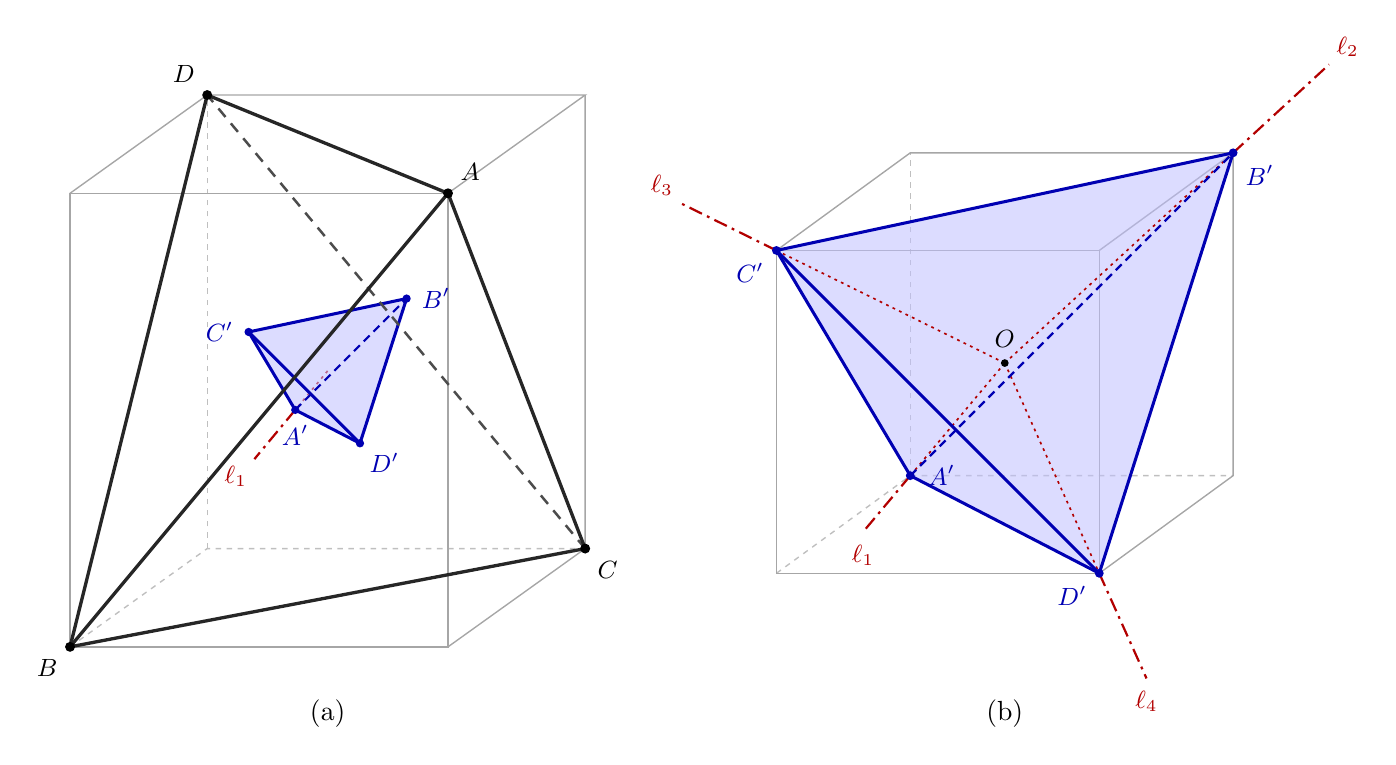
\begin{tikzpicture}[
  boxv/.style={draw=black!35,line width=0.5pt},
  boxh/.style={draw=black!25,line width=0.5pt,dash pattern=on 2pt off 2pt},
  tetv/.style={draw=black!85,line width=1.2pt,line join=round},
  teth/.style={draw=black!70,line width=0.9pt,dash pattern=on 4pt off 3pt},
  morv/.style={draw=blue!70!black,line width=1.1pt,line join=round},
  morh/.style={draw=blue!70!black,line width=0.8pt,dash pattern=on 3pt off 2pt},
  axis/.style={draw=red!70!black,line width=0.8pt,dash pattern=on 5pt off 2pt on 1pt off 2pt},
  lbl/.style={font=\small}]
% (a) the isosceles tetrahedron ABCD in the box [-a,a]x[-b,b]x[-c,c], a=1.3, b=1.5, c=1.8,
%     with a regular Morley tetrahedron, A' = -s(1,1,1), s = 0.4419
\begin{scope}[x={(-0.67cm,-0.48cm)},y={(1.6cm,0cm)},z={(0cm,1.6cm)}]
\def\a{1.3}\def\b{1.5}\def\c{1.8}\def\s{0.44189}
\coordinate (A) at (\a,\b,\c);
\coordinate (B) at (\a,-\b,-\c);
\coordinate (C) at (-\a,\b,-\c);
\coordinate (D) at (-\a,-\b,\c);
\coordinate (A1) at (-\s,-\s,-\s);
\coordinate (B1) at (-\s,\s,\s);
\coordinate (C1) at (\s,-\s,\s);
\coordinate (D1) at (\s,\s,-\s);
\draw[boxh] (\a,-\b,-\c) -- (-\a,-\b,-\c) -- (-\a,\b,-\c);
\draw[boxh] (-\a,-\b,-\c) -- (-\a,-\b,\c);
\draw[boxv] (\a,\b,\c) -- (\a,\b,-\c) -- (\a,-\b,-\c) -- (\a,-\b,\c) -- cycle;
\draw[boxv] (\a,\b,\c) -- (-\a,\b,\c) -- (-\a,-\b,\c) -- (\a,-\b,\c);
\draw[boxv] (\a,\b,-\c) -- (-\a,\b,-\c) -- (-\a,\b,\c);
\draw[red!70!black,line width=0.6pt,dash pattern=on 1pt off 1.6pt] (0,0,0) -- (A1);
\draw[axis] (A1) -- (-1.0,-1.0,-1.0) node[lbl,below left=-1pt,text=red!70!black] {$\ell_1$};
\fill[blue!25,opacity=0.55] (A1) -- (C1) -- (B1) -- (D1) -- cycle;
\draw[morh] (A1) -- (B1);
\draw[morv] (A1) -- (C1) -- (B1) -- (D1) -- cycle;
\draw[morv] (C1) -- (D1);
\foreach \P in {A1,B1,C1,D1} \fill[blue!70!black] (\P) circle (1.5pt);
\node[lbl,below=2pt,text=blue!70!black] at (A1) {$A'$};
\node[lbl,right=2pt,text=blue!70!black] at (B1) {$B'$};
\node[lbl,left=2pt,text=blue!70!black] at (C1) {$C'$};
\node[lbl,below right=0pt,text=blue!70!black] at (D1) {$D'$};
\draw[teth] (C) -- (D);
\draw[tetv] (A) -- (B) -- (C) -- cycle;
\draw[tetv] (A) -- (D) -- (B);
\foreach \P in {A,B,C,D} \fill[black] (\P) circle (1.8pt);
\node[lbl,above right=1pt] at (A) {$A$};
\node[lbl,below left=1pt] at (B) {$B$};
\node[lbl,below right=1pt] at (C) {$C$};
\node[lbl,above left=1pt] at (D) {$D$};
\end{scope}
\node[font=\normalsize] at (0,-4.35) {(a)};
% (b) the Morley tetrahedron: alternate vertices of a cube centred at O; each vertex lies on one of the lines l_i
\begin{scope}[xshift=8.6cm,yshift=0.1cm,x={(-0.85cm,-0.62cm)},y={(2.05cm,0cm)},z={(0cm,2.05cm)}]
\draw[boxh] (1,-1,-1) -- (-1,-1,-1) -- (-1,1,-1);
\draw[boxh] (-1,-1,-1) -- (-1,-1,1);
\draw[boxv] (1,1,1) -- (1,1,-1) -- (1,-1,-1) -- (1,-1,1) -- cycle;
\draw[boxv] (1,1,1) -- (-1,1,1) -- (-1,-1,1) -- (1,-1,1);
\draw[boxv] (1,1,-1) -- (-1,1,-1) -- (-1,1,1);
\fill[blue!25,opacity=0.55] (-1,-1,-1) -- (1,-1,1) -- (-1,1,1) -- (1,1,-1) -- cycle;
\foreach \P in {(-1,-1,-1),(-1,1,1),(1,-1,1),(1,1,-1)} \draw[red!70!black,line width=0.6pt,dash pattern=on 1pt off 1.6pt] (0,0,0) -- \P;
\draw[axis] (-1,-1,-1) -- (-1.5,-1.5,-1.5) node[lbl,below=1pt,text=red!70!black] {$\ell_1$};
\draw[axis] (-1,1,1) -- (-1.42,1.42,1.42) node[lbl,above right=-1pt,text=red!70!black] {$\ell_2$};
\draw[axis] (1,-1,1) -- (1.42,-1.42,1.42) node[lbl,above left=-1pt,text=red!70!black] {$\ell_3$};
\draw[axis] (1,1,-1) -- (1.5,1.5,-1.5) node[lbl,below=1pt,text=red!70!black] {$\ell_4$};
\draw[morh] (-1,-1,-1) -- (-1,1,1);
\draw[morv] (-1,-1,-1) -- (1,-1,1) -- (-1,1,1) -- (1,1,-1) -- cycle;
\draw[morv] (1,-1,1) -- (1,1,-1);
\fill[black] (0,0,0) circle (1.4pt);
\node[lbl,above=2pt] at (0,0,0) {$O$};
\foreach \P in {(-1,-1,-1),(-1,1,1),(1,-1,1),(1,1,-1)} \fill[blue!70!black] \P circle (1.6pt);
\node[lbl,right=3pt,text=blue!70!black] at (-1,-1,-1) {$A'$};
\node[lbl,below right=1pt,text=blue!70!black] at (-1,1,1) {$B'$};
\node[lbl,below left=1pt,text=blue!70!black] at (1,-1,1) {$C'$};
\node[lbl,below left=1pt,text=blue!70!black] at (1,1,-1) {$D'$};
\end{scope}
\node[font=\normalsize] at (8.6,-4.35) {(b)};
\end{tikzpicture}
\end{document}
